\chapter{Training the Dialogue Manager with RL}
\label{chapter:dm-rl}

In the previous chapter, we saw that a fully-operational \acrfull{DS} is a complex pipeline including several sub-modules. But, this thesis being focused on the \acrfull{DM},
%knowing that only one of them, the \acrfull{DM}, will be discussed in the rest of this manuscript,
we will abstract all the remaining \acrshort{DS} modules, and the \idx{user}, into a single entity called the \idx{environment}.
The training of a \acrshort{DS} will hence simplify, without loss of generality, into the optimisation of a \acrfull{DP} interacting with this "augmented" environment.
%we were able to abstract all the remaining modules, including the \idx{user}, into a single module called the \idx{environment}. That means, for our setting, that optimising a \gls{DS} amounts to optimising a \gls{DP} interacting with an \idx{environment}.
%
From now on, we state an equivalence between an \idx{environment} and a \idx{user} and just forget all the other modules.

Usually, in \idx{dialogue} applications, particularly with \idx{task-oriented} \idx{dialogue} applications, the system must keep track of the history of the \idx{dialogue}. If we keep the whole \idx{dialogue} history in the \idx{dialogue state} 
%${\state}_{\indextransition}$,
$s_{\indextransition}$, % TU: je renonce au "s" dans les symboles
the \gls{DP} has all the information it needs to take the better decision at time $\indextransition$ in order to complete the dialogue task:
the \idx{dialogue} state representation is said \textit{Markovian}; more formally, the past states have no additional information to predict the future. Then, in order to keep track of the \idx{dialogue}, the \gls{DM} must update its state according to the previous state and the current observation raised by the \idx{dialogue} using the \acrfull{DST} module. Considering that an observation is conditioned on the current state and the \idx{dialogue act}, then we have enough elements to represent the dynamics of the \idx{environment}, denoted as the transition kernel $\transition$.
Knowing that taking an action given a state leads to another state is helpful to predict multiple steps ahead \textit{i.e.} which state the \gls{DP} may reach if it follows a series of \idx{dialogue act}s. However, it will not suffice to evaluate the policy. To that end, we add a new signal, the immediate reward function, denoted as $\reward$, that indicates how good was a \idx{dialogue act} transitioning from one state to another. By compiling all those information, we are able to optimise the \gls{DP} using a mathematical framework called \acrlong{MDP}~\parencite{bellman57}.

\paragraph{Markov Decision Processes}

We first introduce the core concepts used in this manuscript.

\begin{definition}
    A \acrfull{MDP} is a tuple $\langle{}\cS,\cA,\reward,\transition,\discountfactor\rangle{}$ where:
    \begin{itemize}
        \item  $\cS$ is the state set,
        \item  $\cA$ is the action set,
        \item $\reward\in\Real^{\cS \times \cA}$ is the reward function,
        \item $\transition\in \cM(\cS)^{\cS \times \cA}$ is the transition kernel; $\cM(\cX)$ denotes the probability measure over a set $\cX$.
        \item $\discountfactor$ is the discount factor.
    \end{itemize}
    \label{def:mdp}
\end{definition}

In the \idx{dialogue} context, it may be hard to define a good reward function. For example in chit-chat applications, how to know if a conversation went well for the \idx{user}? Knowing this answer implies using sentiment analysis which is not reliable in the current state-of-the-art. Manual labeling may work, but it requires a costly human labor. Even in those cases, one cannot really decide whether a \idx{user} enjoyed the conversation without asking explicitly \idx{user}s to give feedback\footnote{Even with explicit surveys, there are several biases that must be corrected.}.

For task-oriented situation, if the task is completed, then the \idx{environment} should yield a reward (usually discounted with respect to the length of the dialogue). In simulation, it is easy to know if the task is completed, but in real application, the agent might understood wrongly the request; a lot a work has been done to takcle this issue~\parencite{elasri2016}.

\begin{figure}
    \begin{center}
        \subfloat[][A generic discrete Markov Decision Process. The state $s_2$ is final.]{
        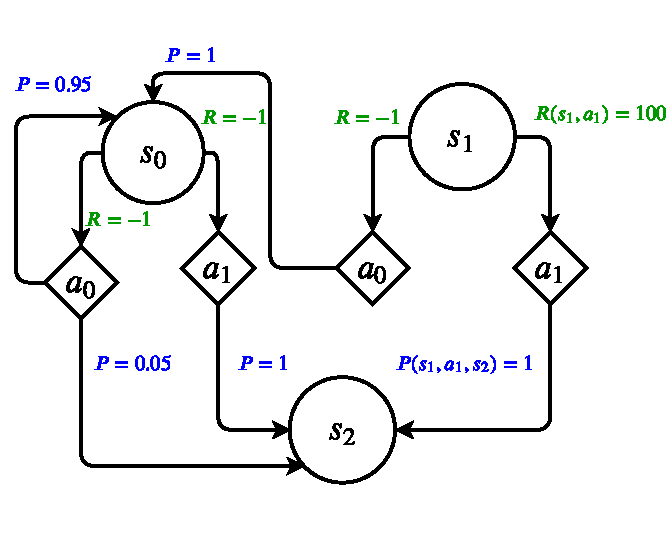
\includegraphics[width=0.5\textwidth]{sources/dm-rl/mdp}
        \label{fig:generic-mdp}
        }\\
        \subfloat[][A Markov Decision Process in a \idx{slot-filling} \idx{dialogue} task. Dashes indicate potentially infinite possibilities of states, transitions and actions.]{
        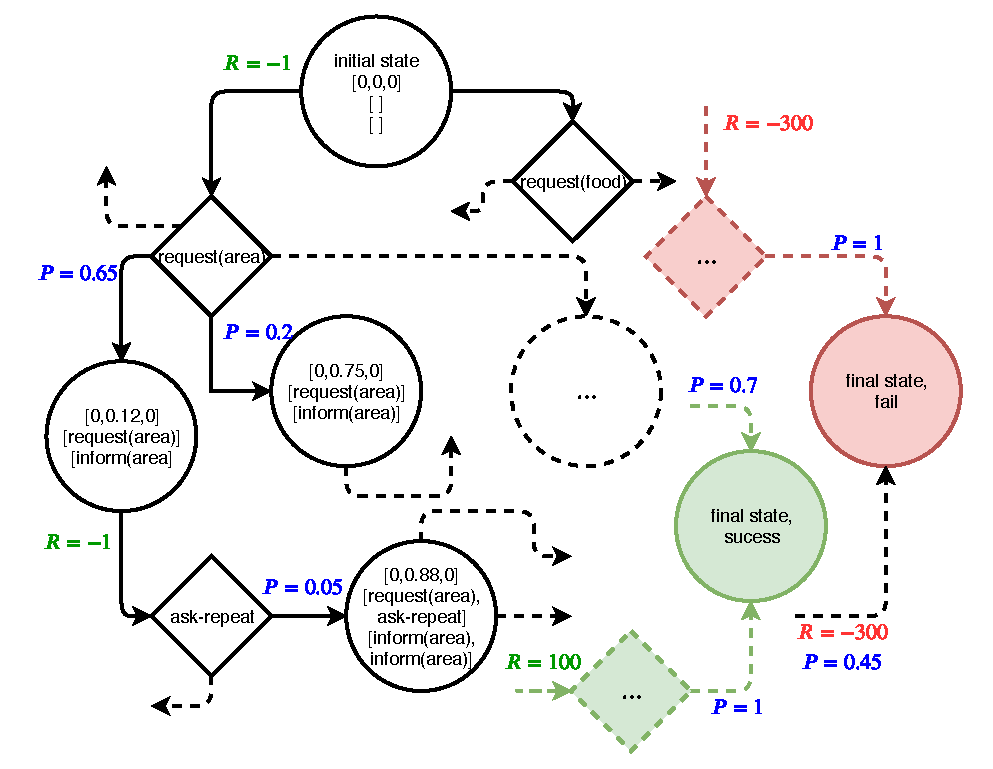
\includegraphics[width=0.7\textwidth]{sources/dm-rl/slot-filling-mdp}
        \label{fig:dm-mdp}
        }
        \caption{Example of Markov Decision Processes}
        \label{fig:renonculacees}
    \end{center}
\end{figure}
%
The state of an \gls{MDP} must contain all past observations. In other words, the \idx{agent} would not be able to take a better decision with additional past information to complete the dialogue task. We say that the process respects the Markov property (or that it is \textit{Markovian}).
\begin{definition}
    Let $(\Omega,\bbP)$  a probability space. Then a \idx{stochastic} process $X=\{X_{\indextransition}\}_{\indextransition\in\T}$ is said to possess the Markov property if
    \begin{equation}
        \mathbb{P}(X_{\indextransition}=x_{\indextransition}|X_{\indextransition-1} = x_{\indextransition-1},\dots,X_0=x_0)=\mathbb{P}(X_{\indextransition}=x_{\indextransition}| X_{\indextransition-1}=x_{\indextransition-1}).
    \end{equation}
\end{definition}
In the context of an \gls{MDP}, that means:
\begin{equation}
    \transition(s_{\indextransition},a,s_{\indextransition+1}) = \mathbb{P}(s_{\indextransition+1}|s_{\indextransition},a) = \mathbb{P}(s_{\indextransition+1}|s_{\indextransition},\dots,s_{0},a).
\end{equation}
For example, if the \idx{agent} is a car, in order to decide how to slow down when it faces another car, it must know its current speed, its position and the position of the other car. If the \idx{agent} only knows its current position and not all other past positions, it will not be able to know its speed and the process will not be \textit{Markovian}.

\Cref{fig:generic-mdp} shows an example of a generic \gls{MDP} illustrating \Cref{def:mdp} side by side with \Cref{fig:dm-mdp}, a partial view of an \gls{MDP} from a \idx{slot-filling} \idx{task-oriented} \idx{dialogue} application. The particularity of an \gls{MDP} in the \idx{dialogue} context is that the state space is actually infinite as the \acrfull{SRS} is a continuous variable. We also note that by keeping all the past \idx{dialogue act}s, \idx{user} acts and the last \gls{SRS} for each slot in the \idx{dialogue state}, we respect the Markov property. Indeed, there is no interest in keeping all the \gls{SRS} from previous utterances as the only thing that matters: whether the system understood correctly a given slot. However, keeping all the past \glspl{SRS} may be useful in a situation where the \idx{dialogue act} includes the value of the slot. For example, if the \idx{user} responds to a \texttt{request(area)} by two \texttt{inform(area=Paris)} with \gls{SRS} 0.7 and 0.9 and one \texttt{inform(area=London)} with \gls{SRS} 0.3, it seems probable that the actual informed area is Paris.

The behaviour of the \idx{dialogue} \idx{agent}, the \gls{DP}, is then defined as the policy $\policy\in\cM(\cA)^{\cS}$, that maps states to actions, which can either be deterministic\index{deterministic policy} or stochastic\index{stochastic policy}. Solving an \gls{MDP} consists in finding a \idx{policy} $\optimalpolicy$ that maximises the amount of rewards gathered by walking on the \gls{MDP}. Usually the objective is to maximise the infinite-horizon $\discountfactor$-discounted sum of rewards, called return, in expectation:

\begin{definition}
    Let $\discountfactor \in [0,1[$, then the $\discountfactor$-discounted return for the policy $\policy$ is
    \begin{align}
        &\return^{\policy} = \sum_{\indextransition=0}^\infty \discountfactor^{\indextransition} \reward(s_{\indextransition},a_{\indextransition})\\
        & \text{where } s_{\indextransition+1} \sim \transition(s_{\indextransition},a_{\indextransition},s_{\indextransition+1}) \text{and } a_{\indextransition} \sim \policy(s_{\indextransition}).\nonumber
    \end{align}
\end{definition}

From a \idx{task-oriented} \idx{dialogue} perspective, it may be strange to consider intermediate rewards. After all, the sole completion of the task matters, but usually, we also want to solve the task as fast as possible. For that purpose, there are two solutions to the \idx{agent} designer (not mutually exclusive): yield a negative reward at each \idx{turn} of the \idx{dialogue} or set a $\discountfactor$ strictly smaller than $1$ to account for the hazard of the user terminating the dialogue at each turn~\parencite{Fedus2019}. In both cases, the longer the \idx{dialogue} lasts, the lower the return will be. One may notice that anyway, for most of the following \gls{RL} theory to apply, one needs the condition $\discountfactor < 1$. %That's not necessarily true as in \idx{task-oriented} application, usually, the number of \idx{turn}s is capped, so algorithms may still converge.

From the return, one can derive the action-value function, also known as $\Q$-function. This function yields the expected return after taking an action in a given state and thereafter following a fixed \idx{policy} $\policy$.

\begin{definition}
    Let $a\in\cA$ and $s\in\cS$ and $\policy$ a \idx{policy}, then
    \begin{align}
        \Q^{\policy}(s,a)=\mathbb{E}_{\policy} [\return^{\policy}|s_0=s,a_0=a].
    \end{align}
\end{definition}

Thanks to the \idx{Bellman Evaluation} equation, we are able to compute the expected return of a \idx{policy} using a simple linear system of equations:

\begin{proposition}
    Let $\policy$ be a \idx{policy}, then $\forall s\in\cS$ and $\forall a\in\cA$.
    \begin{align}
        \Q^{\policy}(s,a)=\reward(s,a) + \discountfactor\sum_{s'\in \cS}[\transition(s,a,s') \sum_{a'}\policy(a'|s')\Q^{\policy}(s',a')].
        \label{eq:bellman-evalutation}
    \end{align}
\end{proposition}

\idx{Bellman Evaluation} equation can be reformulated as $\Q^{\policy}=\bo^{\policy}\Q^{\policy}$ where $\bo^{\policy}$ is the \idx{Bellman Evaluation} operator. Being able to evaluate a \idx{policy} is one thing, but what we really want is finding the best \idx{policy} {w.r.t.} the expected return. We call \idx{optimal} \idx{policy} $\optimalpolicy$, a \idx{policy} that maximises the return in expectation \textit{i.e.}

\begin{definition}
    The \idx{policy} $\optimalpolicy$ is said \idx{optimal} if and only if
    \begin{align}
        \forall (s,a) \in \cS\times\cA,\Q^{\optimalpolicy} (s,a) = \max_{\policy}\Q^{\policy} (s,a).
    \end{align}
\end{definition}

We now present the \idx{Bellman Optimality} equation (or control equation) ~\parencite{Bellman}:
\begin{theorem}{\idx{Bellman Optimality} equation}:
    It exists a unique function, denoted as $\Q^*$, that verifies the \idx{Bellman Optimality} equation:
    \begin{align}
        \Q^*(s,a)=\reward(s,a) +\discountfactor \sum_{s'\in \cS}[\transition(s,a,s')\max_{a'\in \cA}\Q^*(s',a')].
        \label{eq:bellman-control}
    \end{align}
\end{theorem}

\idx{Bellman Optimality} equation can be reformulated as $\Q^*=\bo^{*} \Q^*$ where $\Q^*$ is the \idx{optimal} $\Q$-function and $\bo^{*}$ the \idx{Bellman Optimality} operator (also know as dynamic programming operator). An important property is that we can construct an \idx{optimal} \idx{policy} as an expression of $\Q^*$:
\begin{proposition}
    The \idx{policy} defined by
    \begin{align}
        \optimalpolicy(s) \in \argmax\limits_{a\in \cA} \Q^*(s,a)
    \end{align} is \idx{optimal}.
\end{proposition}
All those results allow us construct algorithms that find this \idx{optimal} \idx{policy}.

\paragraph{Solving with dynamic programming}

If $\discountfactor < 1$, the operator $\bo^{*}$ is a contraction. Thanks to the Banach theorem~\parencite{Banach1922}, it admits a unique solution. Then, one can find $\Q^*$ by iterating on \Cref{eq:bellman-control}: the algorithm is called \gls{VI}~\parencite{bellman57} and recalled on \Cref{alg:value-iteration}.

\begin{algorithm}
    \DontPrintSemicolon
    \KwData{an MDP $\langle{}\cS,\cA,\reward,\transition,\discountfactor\rangle{}$}
    $\n\leftarrow 0$\;
    $\Q_{\n}\in \mathbb{R}^{|\cS\times\cA|}$\;
    \While{$\n=0 \vee ||\Q_{\n+1} - \Q_{\n}|| < \deltastoppingcriterion$}{
    $\Q_{\n+1} \leftarrow  \bo^{*} \Q_{\n}$\;
    $\n \leftarrow  \n+1$;
    }
    $\policy(s) \in \argmax_{a\in\cA} \Q_{\n}(s,a)\ \forall s\in\cS$\;
    \Return $\policy$\;
    \caption{Value-Iteration}
    \label{alg:value-iteration}
\end{algorithm}

Another approach is to evaluate the \idx{policy} with \Cref{eq:bellman-evalutation}, then improve it greedily over the current $Q$-function of the policy. The algorithm is called \gls{PI}~\parencite{howard60} and is described in \Cref{alg:policy-iteration}. \Cref{th:policy-improvment-theorem} ensures that the algorithm converges to the \idx{optimal} \idx{policy}. \gls{PI} and \gls{VI} are quite similar. One difference is that \gls{VI} does evaluation and policy improvement at the same time. The mattering difference is the stopping criterion: \gls{PI} stops once the \idx{policy} has converged which happens earlier than the convergence of the $\Q$-function in \gls{VI}.

\begin{algorithm}
    \DontPrintSemicolon
    \KwData{an MDP $\langle{}\cS,\cA,\reward,\transition,\discountfactor\rangle{}$}
    $\n\leftarrow 0$\;
    $\Q_{\n}\in \mathbb{R}^{|\in\cS\times\cA|}$\;
    $\policy_{\n}$  any \idx{policy}\;
    \While{$\n=0 \vee \policy_{\n+1} \neq \policy_{\n}$}{
    $\Q_{\n+1} = {\bo}^{\policy_{\n}} \Q_{\n}$ (evaluation)\;
    $\policy_{\n+1}(s) \in \argmax_{a\in\cA} \Q_{\n+1}(s,a)\ \forall s\in\cS$ (improvement)\;
    $\n \leftarrow \n+1$\;
    }
    \Return $\policy_{\n}$\;
    \caption{Policy-Iteration}
    \label{alg:policy-iteration}
\end{algorithm}

\begin{theorem}{(Policy Improvement Theorem)}:
    Let $\policy$ a \idx{policy}, $\Q^{\policy}$ its associated $\Q$-function and $\policy'$ defined as :
    \begin{align}
        &\forall s\in\cS, \policy'(s)\in \argmax_{a\in\cA} (\reward(s,a) + \discountfactor \mathbb{E}_{s'}[ \transition(s,a,s') \max_{a'\in \cA} \Q^{\policy}(s',a')])\\\nonumber
        & \text{then } \forall (s,a)\in\cS \times \cA,\ \Q^{\policy'}(s,a) \geq \Q^{\policy}(s,a)\\\nonumber
        & \text{with } \ \Q^{\policy'}(s,a) = \Q^{\policy}(s,a) \text{ iif } \Q^{\policy}(s,a) = \Q^{\optimalpolicy}(s,a).
    \end{align}
    \label{th:policy-improvment-theorem}
\end{theorem}

\paragraph{On the continuous state-space problem}

As we already mentioned, the state-space $\cS$ in the \idx{dialogue} context is actually infinite since the \gls{SRS} is a continuous variable. The tabular solutions of \gls{VI} and \gls{PI} are then intractable. To overcome this issue, we build an approximation of the $\Q$-function. Let $\cF$ be the set of representable functions with domain $\cS\times\cA$, $|| \cdot ||_{\infty}$ the uniform norm, and $\projection$ the projection operator onto $\cF$:
\begin{align}
    \projection f = \argmin_{\tilde{f}\in \cF} || f - \tilde{f} ||_{\infty}.
\end{align}
This process is known as function approximation and is heavily used in today \gls{RL} algorithms. We can naturally extend \gls{VI} to \gls{FVI} (or \gls{AVI}, ~\textcite{bellman59}) using a composition of the \idx{optimal} Bellman operator\index{Bellman Optimality} with the projection operation. In a nutshell, the algorithm iterates over the following contraction\footnote{if the projection is considered perfect, i.e has no bias.}: $\Q^* = \projection\bo^{*} \Q^*$. Projection is usually done by sampling $\tilde{\cS}\subset \cS$ a finite subset of $\cS$ and then process a \idx{regression} over the learning examples $ \tilde{\cS}\times \cA$. Let $\Gamma (X,Y): \rightarrow \cF$ denotes the \idx{regression} algorithm, then the update rule is as follows:
\begin{align}
    &\Q^* \leftarrow \Gamma(\tilde{\cS}\times \cA,\{\bo^{*} \Q^*(x)\}_{x\in \tilde{\cS}\times \cA}).
\end{align}
If we apply the same idea to \gls{PI} (on the evaluation only), we obtain \gls{API}~\parencite{bertsekas1996}. Please note that the \idx{regression} algorithm can take various forms, as for example linear \idx{regression}, \idx{regression} trees or even \acrlong{NN}s.

\paragraph{Toward Reinforcement Learning solutions for Dialogue Systems}

\begin{figure}
    \begin{center}
        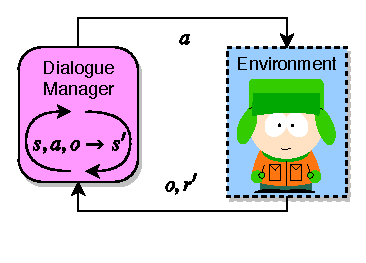
\includegraphics[width=0.7\textwidth]{sources/dm-rl/rl-pipeline}
        \caption{\label{fig:rl-pipeline} The Dialogue Manager cast as a Reinforcement Learning problem.}
    \end{center}
\end{figure}

Another problem arises when dealing with \idx{dialogue} applications. The function $\reward$ and $\transition$ are actually determined by the \idx{user} (and the plugged pipeline) the system \idx{dialogue}s with. That means that $\reward$ and $\transition$ correspond to a \idx{model} of the \idx{user}, which is complex, unknown and varies a lot from one individual to another.
%
So in a the \idx{dialogue} context, $\reward$ and $\transition$ must be learnt (or implicitly learnt) using information on the \idx{user}. \gls{RL} allows to handle this flow of information. \gls{RL} is a framework used to describe an \idx{agent} (e.g. the \gls{DM}) interacting with an \idx{environment} (e.g. the \idx{user} and peripheral modules) in a sequential fashion. The \gls{DS} pipeline is cast as an \gls{RL} problem in \Cref{fig:rl-pipeline}. The information contained in an interaction can be compiled into a single object called \idx{transition}. This is a tuple of the form: $(s, a, s', r')$ where $s$ is the state of \idx{agent}, $a$ the action applied on the \idx{environment}, $r'$ the reward received from the \idx{environment} and $s'$ the next state of the \idx{agent}. A \idx{batch} $\cD$ (a \idx{dialogue corpus}) is a collection of $\T$ \idx{transition}s: $\cD = \{(s_{\indextransition},a_{\indextransition},s'_{\indextransition},r'_{\indextransition})\}_{i\in \left[0,\T \right[}$.

Two classes of problems arise depending on how this information is gathered: on one hand, in \idx{Online} \gls{RL}, the objective is to learn on-the-fly a \idx{policy} using the flow of \idx{transition}s. On the other hand, in \idx{Offline} (or Batch\index{batch}) \gls{RL}, the objective is to directly learn a \idx{policy} given a \idx{batch} $\cD$. In the next sections, we introduce algorithms from both categories that have been successfully applied to \gls{DM}. We start with Batch\index{batch} \gls{RL}.

\section{Assuming a given dialogue corpus}

Dialogue\index{dialogue} applications involving statistical methods usually assume that the \idx{dialogue corpus} is given. A panel of \idx{dialogue} datasets are available for research. To name the famous ones, there is the Ubuntu \idx{dialogue} corpus~\parencite{Lowe2015-ubuntu-corpus} and the \gls{DSTC} dataset~\parencite{dstc}. Please refer to ~\textcite{serban2015-survey-dialogue-corpora} for an extended overview. Usually, the challenge in using dialogue corpora\index{dialogue corpus} for \gls{RL} context is the design of the reward, but this is not the focus here in the thesis, so we assume having a well-formed \idx{dialogue corpus}; as stated earlier, we denote it as a \idx{batch} of \idx{transition}s: $\cD = \{(s_{\indextransition},a_{\indextransition},s_{\indextransition}',r_{\indextransition}')\}_{{\indextransition}\in [0,\T]}$. In \idx{model-based} approaches, we explicitly learn the unknown functions $\transition$ and $\reward$ using a \idx{regression} algorithm and $\cD$ as learning \idx{batch}, then apply a planning algorithm~\parencite{Lison2013ModelbasedBR, peng2018deep}. In \idx{model-free} \idx{batch} \gls{RL}, we do not explicitly estimate $\reward$ and $\transition$ but we can, among other methods, bootstrap the estimation of $\Q$ with the current reward $r$ and the expected reward in the next state $s'$. For example, in \gls{FTQ}~\parencite{Ernst05,Riedmiller05}, in addition to the projection operator, we apply a sampled \idx{Bellman Optimality} operator on the \idx{batch}:

\begin{definition}
    Let $(s,a,s',r')$ be a \idx{transition}, and $f:\cS\times\cA\rightarrow\mathbb{R}$ a function. The Sampled Bellman Optimality\index{Bellman Optimality} operator $\hat{\bo^{*}}$ is :
    \begin{align}
        \hat{\bo^{*}}(f(s,a)) = r' + \discountfactor  \max_{a'\in\cA} f(s',a').
    \end{align}
\end{definition}

The general \gls{FTQ} algorithm (\Cref{eq:fitted-q}) is then an interactive process over the composed operator: $\Q^* = \projection\hat{\bo^{*}} \Q^*$ with respect to $\cD$.
\begin{align}
    &\Q^* \leftarrow \Gamma(\{s_{\indextransition},a_{\indextransition}\}_{{\indextransition}\in \T},\{r'_{\indextransition} + \discountfactor  \max_{a'\in\cA} \Q^*(s'_i,a')\}_{{\indextransition} \in \T}).
    \label{eq:fitted-q}
\end{align}
As in \gls{FVI}, the designer is free to choose the \idx{regression} algorithm suitable to his problem. Trees~\parencite{Ernst05} and \glspl{NN}~\parencite{Riedmiller05} have been successfully combined with general \gls{FTQ}. If using a \gls{LS} linear-regression, the $\Q$-function can be rewritten as
\begin{equation}
    \Q_{ \params}(s,a)=  \params^{\transpose}\features(s,a),
\end{equation}
with $\features$  the \idx{feature} function and $\params$ the parameter to find. Linear \gls{LS} optimisation results in computing $\params$ with a simple matrix inversion. Let $M = (\sum_{{\indextransition}=0}^{\T}\features_(s_{\indextransition},a_{\indextransition})\features((s_{\indextransition},a_{\indextransition}))^{\transpose})^{-1}$, then \gls{FTQ} is the following iterative process:
\begin{equation}
    \params_{\n} \leftarrow M \sum_{\indextransition=0}^{\T} \features(s_{\indextransition},a_{\indextransition})(r_{\indextransition}'+\discountfactor\max_{a\in \cA}( \params_{\n-1}^{\transpose} \features(s_{\indextransition}',a))).
\end{equation}

The algorithm stops if $\n \geq \maxiteration$ where $\maxiteration \in [0,\infty[$ the number maximum of iterations, or if $||\params_{\n}-\params_{\n-1}|| \leq \deltastoppingcriterion$.
This solution has been adopted in~\parencite{pietquin2011sample}. The authors chose an \gls{LS} linear-regression with Gaussian radial basis functions as features\index{feature} in order to optimise a \gls{DM}.

We can extend \gls{PI} using the same idea applied to the \idx{Bellman Evaluation} operator. The algorithm is called \gls{LSPI}~\parencite{Lagoudakis03} and has been applied to \idx{dialogue} tasks~\parencite{li2009reinforcement,barlier18}.

%

\section{Online interactions with the user}

Creating a fixed \idx{dialogue corpus} is a difficult task. 
A dialogue is by essence an interactive and evolving process, and the existing corpora may be too expensive or even not suited for the problem at hands.
In consequence, in some situations, it may be of interest to simply learn, or adapt, on-the-fly the \gls{DM} strategy while it \idx{dialogue}s with an unknown \idx{user}/\idx{environment}. In this section, we present algorithms to do such interactions with the \idx{user} ~\parencite{Ferreira2013}. Those methods belong to the class of \idx{Online} \gls{RL} algorithms.

\paragraph{The Exploitation/Exploration dilemma}

For a new user, in order to gather the \idx{transition}s the algorithm will learn with, the \gls{DM} adopts decisions dictated by a \gls{DP} $\policy$ called the \idx{behavioural policy}. In order to learn the optimal \idx{policy} (target \idx{policy}), $\policy$ needs to gather all the \idx{transition}s that would potentially be covered by the optimal \idx{policy}. As we are actually building this \idx{policy}, it is not possible to know in advance the useful \idx{transition}s for learning. The basic idea to cover the state-action space as the optimal \idx{policy} would do it is to perform an \idx{Exploration/Exploitation} strategy. The exploration phase discovers new areas in the state-action space, while the exploitation phase directs the \idx{agent} to a more profitable state-action space. Several implementations of the \idx{Exploration/Exploitation} dilemma have been proposed, coming from the Bandit community most of the time. In this manuscript, we will use the notorious \idx{$\egreedy$-greedy} strategy which works as follows:
when the \idx{agent} is in state $s$, it chooses a random \idx{exploration} action with probability $\egreedy$, and it chooses the \idx{greedy} action (the most profitable action according to some parameters, the $\Q$-function for example) otherwise.

As long as $\policy$ gathers \idx{transition}s, the \idx{policy} in construction (which is not necessarily  $\policy$) tends to be a better approximation of the optimal \idx{policy}. The \idx{agent} must refine its knowledge around the profitable states and for that, the $\egreedy$ must decrease with respect to the number of \idx{transition}s gathered.
Exponential decay is commonly used for such a decreasing processes.
The number $\egreedy$ is then a variable of {${\indextransition}$}, the current number of \idx{transition}s\footnote{or trajectories\index{trajectory}, this does not matter.}: $\egreedy({{\indextransition}}) = \exp(-{\lambda} {{\indextransition}})$ with {$\lambda$} dictating the vanishing speed. But, as the exponential decay procedure does not ensure convergence, it is usually safer to use a linear decay~\parencite{auer2002finite}:
$\egreedy({{\indextransition}}) = \min\{1,1/(\lambda\indextransition)\}$.

Note that we can already see the limitations of this approach for new users; it is not profitable to act randomly with a human discovering a new dialogue system, the risk of abandon is too high. We will see later that we can handle this issue with \gls{TL}.


\paragraph{On-policy versus Off-policy}

\idx{Online} \gls{RL} algorithms can be classified into two subcategories depending on the nature of the behavioural \idx{policy}. If the algorithm improves this \idx{policy} as it gathers \idx{transition}s, then we say the algorithm is \idx{On-policy}. If the algorithm optimises a \idx{policy} distinct from the behavioural \idx{policy}, then we say the algorithm is \idx{Off-policy}.

The classic \idx{Off-policy} algorithm is $\Q$-learning. It updates the $\Q$-function according to the \gls{TD} error. This error captures the difference between the current estimation of the expected return and the immediate reward summed to the expected return in the next state. The $\Q$-learning is recalled in \Cref{eq:q-learningg}. The hyper-parameter ${\learningrate}$ is the learning rate and ${(s_{\indextransition},a_{\indextransition},s_{\indextransition}',r_{\indextransition}')}$ is the last \idx{transition} {${\indextransition}$} the behavioural policy generated.
\begin{equation}
    \Q({s_{{\indextransition}}}, {a_{{\indextransition}}}) \leftarrow \Q({s_{{\indextransition}}}, {a_{{\indextransition}}})+{\learningrate}[{r'_{{\indextransition}}}+\discountfactor \max _{a'\in\cA} \Q({s'_{{\indextransition}}}, a')-\Q({s_{{\indextransition}}}, {a_{{\indextransition}}})].
    \label{eq:q-learningg}
\end{equation}

To ensure convergence, the learning rate must decrease linearly. $\Q$-learning is not fit to learn the \gls{DP} as it is a tabular solution and as we saw earlier, the \idx{dialogue state} contains continuous variables. In the same spirit of tractability in \idx{Offline} \gls{RL}, one can extend \idx{Online} algorithms using function approximation.

\paragraph{Function approximation}

A straightforward approach adopted for $\Q$-learning is the \gls{LS} \idx{linear-regression} of a \idx{model} of the $\Q$-function using \gls{GD}. The $\Q$-function is approximated with a linear \idx{model}:  $\Q(s,a) = \features(s,a)^{\transpose}\params$ where  $\features$ is the \idx{feature} vector and  $\params$ the parameter vector to optimise. The optimiser is not a \gls{GD} strictly speaking as we regress $\Q$ over the error of a single \idx{transition} rather the whole \idx{batch}. Indeed, the algorithm receives \idx{transition}s one by one, so the optimiser actually used is the \gls{SGD}. The loss $L$ is defined as:
\begin{align}
    L(\params)
    &=\frac{1}{2}({r'_{{\indextransition}}}+\discountfactor \max _{a'\in\cA} \Q({s'_{{\indextransition}}}, a')-\Q({s_{{\indextransition}}}, {a_{{\indextransition}}}))^{2}\\
    &=\frac{1}{2}({r'_{{\indextransition}}}+\discountfactor \max _{a'\in\cA} \features({s_{\indextransition}'}, a')^{\transpose} \params -\features({s_{\indextransition}}, {a_{\indextransition}})^{T} \params)^{2}.
\end{align}
We define $\Q^+ = \discountfactor \max _{a'\in\cA} \features({s_{\indextransition}'}, a')^{\transpose}\params$. Then we compute the gradient of the loss considering $\Q^+$ constant with respect to $\params$. This method is called semi-gradient and is developed as follow:
\begin{align}
    \nabla L(\params) &=
    \nabla\frac{1}{2}({r'_{{\indextransition}}}+ \Q^+ -\features({s_{\indextransition}}, {a_{\indextransition}})^{\transpose} \params)^{2}\\
    &=({r'_{{\indextransition}}}+\Q^{+}-\features({s_{\indextransition}}, {a_{\indextransition}})^{\transpose} \params) \cdot \features({s_{\indextransition}}, {a_{\indextransition}}).
\end{align}
We update $\params$ such that we minimise the loss. The update rule recalled in \Cref{eq:ls-q-learning} defines the \gls{LS} $\Q$-learning algorithm\footnote{In this context, $\indextransition = \n$ as the parameters are updated for each new transition.}:
\begin{align}
    &\params_{\n+1} \leftarrow \params_{\n}-{\learningrate} \nabla L(\params_{\n})\label{eq:ls-q-learning}\\
    &\params_{\n+1} \leftarrow \params_{\n}-{\learningrate} (r'_{\indextransition}+\discountfactor \max _{a'\in\cA} \features(s_{\indextransition'}, a')^{\transpose}\params_{\n} - \features(s_{\indextransition}, a_{\indextransition})^{\transpose} \params_{\n}) \cdot \features(s_{\indextransition}, a_{\indextransition})
\end{align}
\textcite{Riedmiller05} proposed a natural extension to \gls{FTQ} in the \idx{Online} setting; It involves alternating between two phases: it generates a \idx{batch} of \idx{transition}s with an \idx{$\egreedy$-greedy} \idx{policy} using the current target \idx{policy} as the \idx{greedy} component; Then it updates the target \idx{policy} with all previous batches\index{batch}. It repeats this operation until $\egreedy$ decays enough.

\paragraph{Learning from scratch}

In dialogue system applications, it is not usually easy to learn a \gls{DP} from scratch using \idx{Online} \gls{RL} algorithms. Indeed, the first interactions with the user are crucials to build a bond between the service and the user; taking random actions, using $\egreedy$-greedy, to gather information about the environment (including the humain) may just end-up with user dropouts. To tackle this problem, it is possible to contraint the action-space to get the relevant actions for a given state~\parencite{singh2002,williams2008,laroche2009,laroche2010a}. As those solutions necessitate an expertise on \gls{RL}, new studies introduced techniques suited to an average developer; to name a few: \gls{RL} results monitoring~\parencite{laroche2010b}, convergence speed prediction~\parencite{elasri2013} or interaction quality prediction~\parencite{elasri2014}. In this thesis we tackle this problem using \acrfull{TL}, as we will see in the next chapter.
%=======
%In dialogue system applications, it is not usually hard to learn a \gls{DP} from scratch using \idx{Online} \gls{RL} algorithms. Indeed, the first interactions with the user are crucial to build a bond between the service and the user; taking random actions, using $\egreedy$-greedy, to gather information about the environment (including the humain) may just end-up with user dropouts. To tackle such problem, it is possible to contraint the action-space to the relevant ones in a given state~\parencite{singh2002,williams2008,laroche2009,laroche2010a}. As those solutions necessitate an expertise on \gls{RL}, new studies introduced techniques suited to an average developer; to name a few: \gls{RL} results monitoring~\parencite{laroche2010b}, convergence speed prediction~\parencite{elasri2013} or interaction quality prediction~\parencite{elasri2014}. In this thesis we tackle this problem using $\gls{TL}$, as we will see in the next chapter.
%>>>>>>> master

\section{To go beyond}

There exists a lot of solutions in \gls{RL} applied to \gls{DM} that goes beyond the scope of this thesis. Very popular approaches involve \acrfull{DRL}: action-value approximation with \gls{DQN}~\parencite{Mnih2015} used to solve "Settlers of Catan" a negotiation game~\parencite{Cuayhuitl2015StrategicDM}; \gls{PG} methods with REINFORCE~\parencite{Williams1992:REINFORCE} to play the the multi-modal game GuessWhat?!~\parencite{Vries2017-GuessWhat}; Actor-Critic methods with Actor-Critic-Experience-Replay ~\parencite{Wang2016-ACER} have also been applied to the \gls{DM}~\parencite{Weisz2018-ac-rl}.

